\documentclass[a4paper, 10pt]{report}
\usepackage[italian]{babel}
\usepackage[T1]{fontenc}
\usepackage[utf8]{inputenc}
\usepackage{charter}
\usepackage{amsmath}
\usepackage{amsthm}
\usepackage{amsfonts}
\usepackage{graphicx}
\usepackage{wrapfig}
\usepackage{tcolorbox}
\usepackage{fancyhdr}

\usepackage{geometry}
\geometry{a4paper, left=2cm,right=2cm,top=2cm,bottom=2cm}

\pagestyle{fancy}
\lhead{}
\chead{}
\lhead{\bfseries Fondamenti dell'informatica}
\rhead{\bfseries 01 - 07 ottobre 2019}

\begin{document}

\section*{\underline{Teorema di Cantor}}
Uno dei teoremi fondamentali dell'informatica è il teorema di Cantor (1861). Questo teorema afferma che la cardinalità dell'insieme dei numeri naturali è inferiore alla cardinalità dell'insieme delle funzioni che vanno dai numeri naturali ai numeri naturali.\\

\begin{tcolorbox}
	\paragraph{Teorema:}
	\begin{center}
	$|N| < |N \rightarrow N|$
	\end{center}
	
	\paragraph{Dimostrazione:}
	Supponiamo che $|N| = |N \rightarrow N|$. Poichè il numero di funzioni è uguale a quello dei numeri, posso assegnare ad ognuna un indice e ordinarle in base a quello.
	
	Costruisco ora una funzione $g(x) = f_x(x)+1$, ovvero ottenuta prendendo la funzione di indice x e aggiungendoci 1.
	
	Di conseguenza esisterà un numero $\bar{n}$ tale che $g = f_{\bar{n}}$.
	
	Quindi $f_{\bar{n}}(\bar{n}) = g(\bar{n}) = f_{\bar{n}}(\bar{n})$. Questo non è possibile perchè un numero non può essere uguale al suo seguito e quindi si genera un assurdo, che parte dalla supposizione iniziale.\\
	
	Attenzione: la dimostrazione di Cantor vale anche nel caso in cui si abbia $|N \rightarrow {0, 1}|$ -> $g(x) = \bar{f_x(x)}$, quindi se ho vero diventa falso o viceversa. 
\end{tcolorbox}

\paragraph*{Cantor nell'informatica} In informatica il teorema di Cantor può essere utilizzato per suddividere i problemi risolvibili tramite algoritmi da quelli non risolvibili. Infatti permette di dimostrare che che esistono problemi, ovvero funzioni input/output, non
programmabili. Le ipotesi molto deboli del precedente ragionamento lo rendono applicabile
a tutti i linguaggi di programmazione noti.

\section*{\underline{Alfabeti e linguaggi}}
Un \textbf{alfabeto} $\Sigma$ è un insieme finito di simboli (entità astratte non definite). Con $\Sigma^*$ si indica l'insieme costituito da tutte le stringhe su un fissato alfabeto $\Sigma$. La sua cardinalità è pari a quella dei numeri naturali ($|\Sigma^*| = |N|$).

Una \textbf{stringa} (o parola) $\sigma$ è una sequenza finita di simboli uno dietro l’altro. Con le stringhe è possibile eseguire le seguenti operazioni:\\

\begin{tabular}{lp{0.77\textwidth}}
 - Concatenazione: & $\sigma_1 \cdot \sigma_2$. 

Se $\sigma_1$, $\sigma_2 \in \Sigma^*$, allora $\sigma_1 \cdot \sigma_2 \in \Sigma^*$.\\
 - Lunghezza: & $|\cdot| : \Sigma \rightarrow N$

Esempio: $|\sigma_1 \cdot \sigma_2| = |\sigma_1| + |\sigma_2|$. Il simbolo $\varepsilon$ rappresenta la stringa vuota. La lunghezza della stringa vuota ($|\varepsilon|$) è 0.\\\\
\end{tabular}

Un linguaggio (formale) è un insieme di stringhe appartenenti all'insieme delle stringhe corrette $\Sigma^*$ dell'alfabeto $\Sigma$:
\begin{center}
$\mathfrak{L} \subseteq \Sigma^*$ 
\end{center}
Per ogni linguaggio valgono:
\begin{enumerate}
\item $\mathfrak{L}_1, \mathfrak{L}_2 \in \Sigma^*$ 
allora $ \mathfrak{L}_1 \cdot \mathfrak{L}_2 = 
\{ \sigma | \sigma_1 \cdot \sigma_2$ and $\sigma_1 \in \mathfrak{L}_1, \sigma_2 \in \mathfrak{L}_2 \}$ 
\item $\mathfrak{L}_1 \cup \mathfrak{L}_2 = \{ \sigma | \sigma_1 \in \mathfrak{L}_1$ or $\sigma_2 \in \mathfrak{L}_2 \}$ 
\item $\mathfrak{L}^* = \bigcup_{n \in N} \mathfrak{L}^n$
\end{enumerate}


L’insieme vuoto $\emptyset$ e l’insieme \{$\varepsilon$\} sono due linguaggi formali di qualunque alfabeto. Il complemento di un linguaggio $\mathfrak{L}$ è:
\begin{center}
$\bar{\mathfrak{L}} = \{\sigma | \sigma \in \Sigma^* $ and $ \sigma \notin \mathfrak{L} \}$
\end{center}

\begin{tcolorbox}
Definizione matematica di $\Sigma^*$:
$\begin{cases} 
\mathfrak{L}^0 = \{ \varepsilon\} \\
\mathfrak{L}^{n+1} = \mathfrak{L} \cdot \mathfrak{L}^n
\end{cases} $\\

\underline{Esempio}: se $\Sigma = \{a, b \}$ allora $\Sigma^* = \{\varepsilon, a, b, aa, ab, ba, bb, ... \}$.
\end{tcolorbox}

\subsection*{Problema decisionale}
Un problema decisionale può rappresentato tramite il seguente schema:

\begin{center}
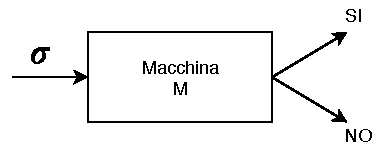
\includegraphics[scale=0.85]{immagine1.pdf}
\end{center}

\noindent La cardinalità dell'insieme degli input è inferiore alla cardinalità dell'insieme dei numeri naturali. Quindi gli input sono un insieme finito \footnote{I numeri naturali sono, in ordine, il primo infinito che si incontra, nonchè il più piccolo. Di conseguenza, tutto ciò che ha cardinalità inferiore è per forza finito.}.
Il linguaggio $\mathfrak{L}$, in questo caso, si definisce come segue:
\begin{center}
$\mathfrak{L} = \{\sigma | f_\mathfrak{L}(\sigma) = 1 \}$
\end{center}

\noindent con $f_\mathfrak{L} \in \Sigma^* \rightarrow \{0, 1 \}$.

\noindent Con la nuova definizione del linguaggio, è possibile riscrivere il problema come segue:

\begin{center}
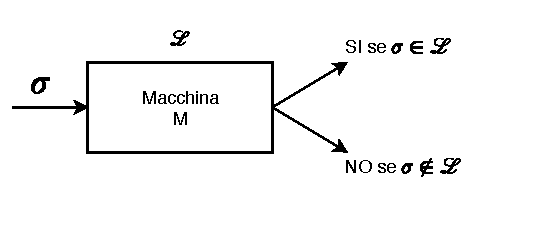
\includegraphics[scale=0.85]{immagine2.pdf}
\end{center}

\end{document}